\RequirePackage[2020-02-02]{latexrelease}
\documentclass[letter,scriptaddress,twocolumn, prl,nofootinbib]{revtex4}

\usepackage{amsmath}%,amssymb} 
\usepackage{makeidx}
\usepackage{amsfonts}
\usepackage[ansinew]{inputenc}
%\usepackage[usenames,dvipsnames]{pstricks}
%\usepackage{subfigure}
\usepackage{epsfig}
\usepackage{float}
%\usepackage{pst-grad} % For gradients
%\usepackage{pst-plot} % For axes
\usepackage[colorlinks,hyperindex]{hyperref}
\hypersetup
{
colorlinks,%
citecolor=black,%
linkcolor=black,%
urlcolor=black,%
}

\setlength\textheight{24.5cm}

% --- Comandos novos ---
\newcommand{\dket}[1]{\left| #1 \right)}
\newcommand{\E}[1]{\frac{\hbar^2 #1 ^2}{2m_0}}
\newcommand{\dbra}[1]{\left( #1 \right|}
\newcommand{\dsubmin}[1]{\left( #1 \right)}
\newcommand{\dbraket}[2]{\left( #1 | #2 \right)}
\newcommand{\dbraketm}[3]{\left( #1 \left| #2 \right| #3 \right)}
\newcommand{\ket}[1]{\left| #1 \right\rangle}
\newcommand{\bra}[1]{\left\langle #1 \right|}
\newcommand{\submin}[1]{\left\langle #1 \right\rangle}
\newcommand{\Var}[1]{\text{Var}\left( #1 \right)}
\newcommand{\braket}[2]{\left\langle #1 \right. \left| #2 \right\rangle}
\newcommand{\braketm}[3]{\langle #1 \mid #2 \mid #3 \rangle}
\newcommand{\pinterno}[2]{\left( #1 , #2 \right)}
\newcommand{\comut}[2]{\left[ #1 , #2 \right]} % THE COMUTATOR
\newcommand{\seitz}[2]{\left\{ \, #1 \mid  #2 \, \right\}}
\newcommand{\rep}{\emph{rep} }
\newcommand{\irep}{\emph{irrep} }
\newcommand{\ordem}[1]{\mid #1 \mid}
\newcommand{\op}[1]{\mathbb #1 }
\newcommand{\group}[1]{\mathcal #1 }
\newcommand{\vet}[1]{\mathbf #1 }
\newcommand{\argu}[1]{\left( #1 \right)}
\newcommand{\kp}{\vet{k}\cdot\vet{p}}

\makeindex

%--------------------------------------------------------
\begin{document}

\title{Computational Simulation of the 2d Ising Model}

\author{Alex Roseman}
\author{Adrian Hall}
\date{\today}

\begin{abstract}
In this paper, we simulate the 2d Ising Model on a square 100 x 100 lattice using the Metropolis-Hastings algorithm. We observe a phase transition, and calculate a critical temperature in agreement with the analytic value. We observe unexpected behavior in the correlations between nearby spin states, which converge to negative values at long distances, likely due to finite-size effects. We calculate critical exponents, which we find outside of error bars.
\end{abstract}

\maketitle

\begin{figure*}[t]
	\begin{center}
		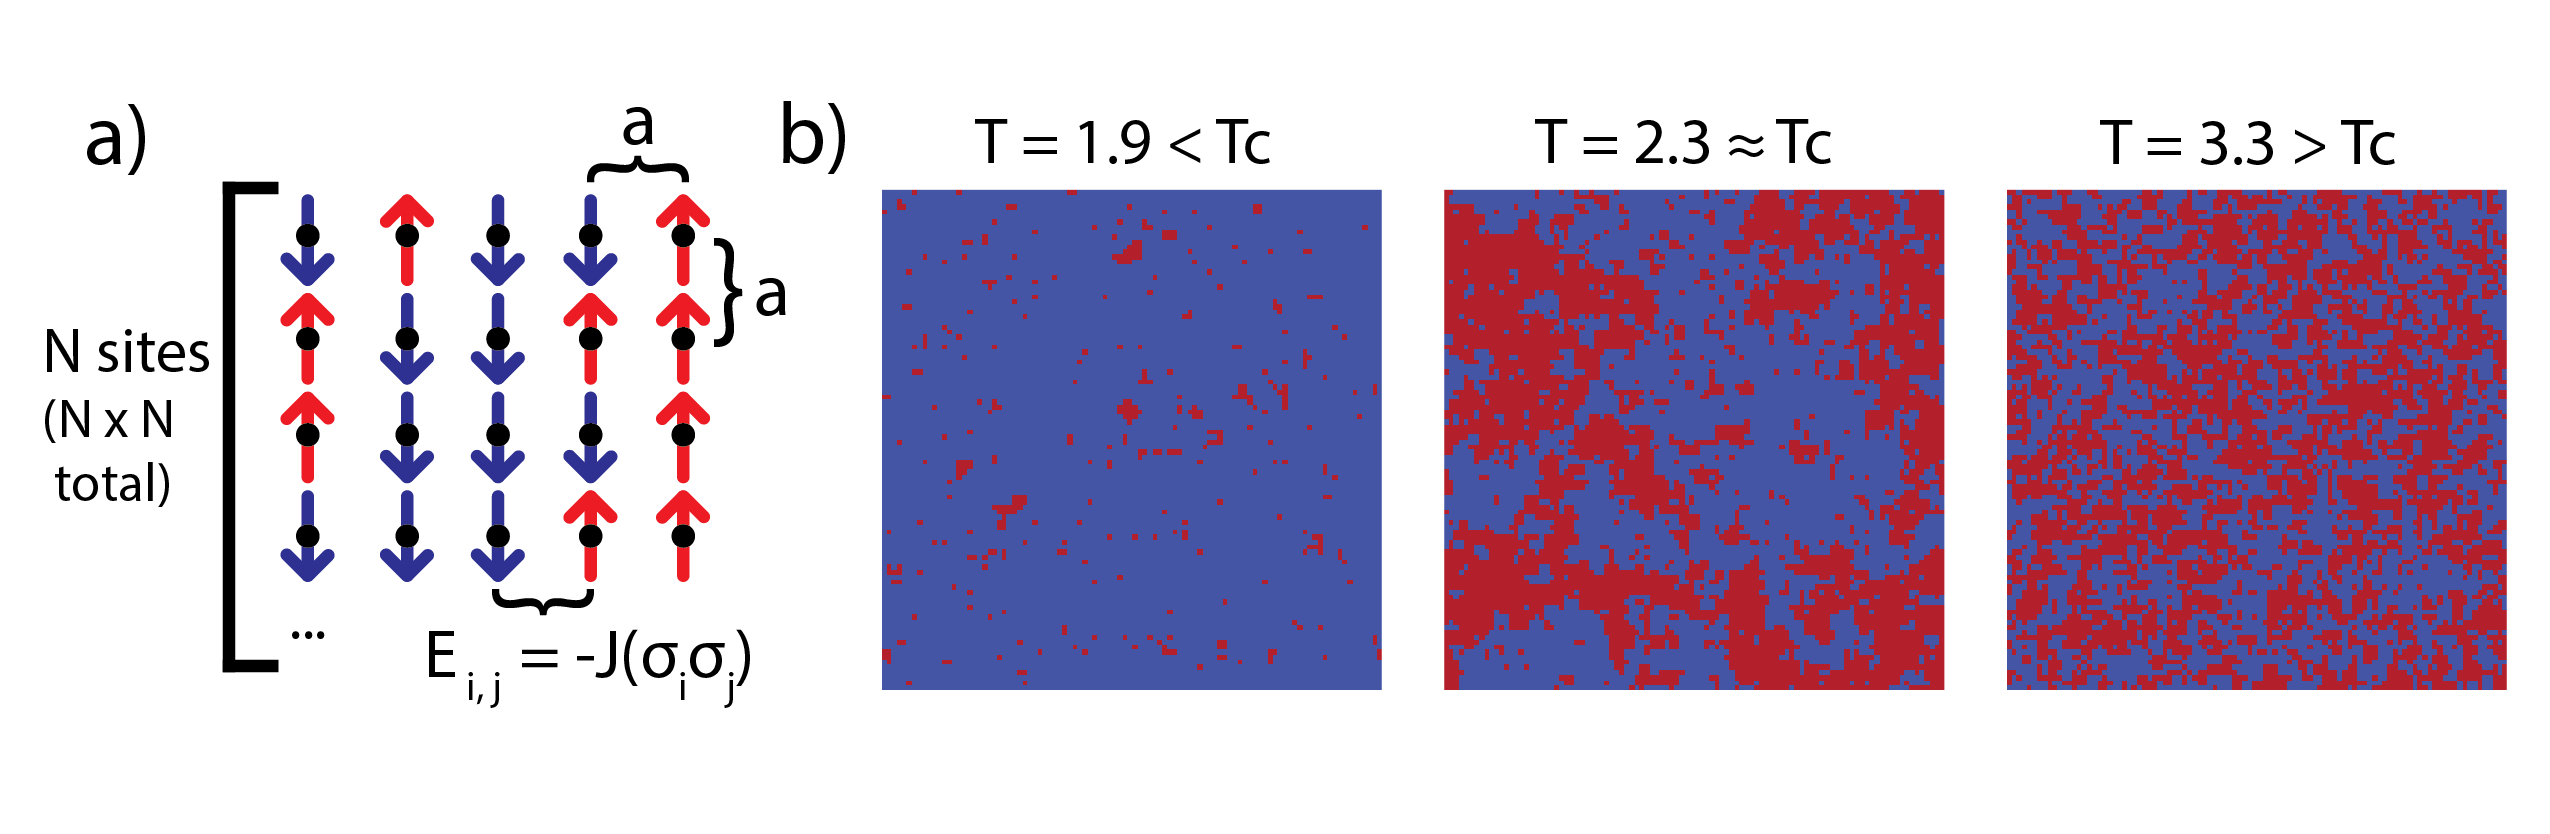
\includegraphics[width=1\textwidth]{figs/fig1.png}
		\caption{a. A diagram of the square lattice. We use lattice size $N = 100$, lattice distance $a = 1$, interaction energy $J = 1$, and spin = $\sigma = \pm 1$ throughout. $E_{i, j}$ is the interaction energy between adjacent spin sites (the lattice wraps around such that each site has 4 neighbors). b. Snapshots after ten million simulation steps at the given temperature, showing typical states below, near, and above Tc. Red squares have spin up, blue squares spin down.}
		\label{fig:fig1}
	\end{center}
\end{figure*}

\textbf{Introduction:} The Ising model is an idealized model of ferromagnetism and notably one of the few models in statistical mechanics with an exact analytical solution. In the model, a solid material is represented as a regular $d$-dimensional lattice of spin states, each of which can take one of two values ($\pm 1$). The spin states interact with their neighbors and with an external magnetic field according to the Hamiltonian
\begin{equation}
	\label{eq:hamiltonian}
	H = -J \sum_{\langle i, j \rangle} \sigma_i \sigma_j - B \sum_i \sigma_i
\end{equation}
where $\sigma_i$ is the magnetic moment at lattice site $i$, $J$ is the interaction energy, $B$ is the magnetic field strength, and $\langle i, j \rangle$ denotes all pairs of neighboring lattice sites.

Onsager's analytical solution for infinite rectangular lattices \cite{Onsager} describes the equilibrium behavior of the model as a function of $J$ and $B$ as well as the temperature $T$. An interesting feature is that on a lattice that is infinite in two dimensions, the model exhibits a phase transition at the critical temperature $T_c$, given by
\begin{equation}
	\label{eq:Tc}
	\frac{k_B T_c}{J} = \frac{2}{\ln{(1+\sqrt{2})}} \approx 2.269
\end{equation}
where $k_B$ is Boltzmann's constant. At $T_c$ the equilibrium state of the model is discontinuous with respect to temperature. Qualitatively, for $T > T_c$ the lattice is highly disordered, while for $T < T_c$ the spin states correlate significantly with others nearby (\autoref{fig:fig1}).

The model's behavior at temperatures near $T_c$ has been the subject of extensive study. As the temperature approaches $T_c$, several observable quantities vary according to power laws in the reduced temperature $t = \frac{T - T_c}{T_c}$. Among these are specific heat $C_v$, absolute magnetization $|M|$, magnetic susceptibility $\chi$, and correlation length $\xi$. Auto-correlation $\submin{\sigma(0)\sigma(x)}$ also varies according to a power law, although in lattice distance $x$ rather than in $t$. These power laws, and their corresponding exponents (the critical exponents) are not specific to a particular Ising lattice; rather, they are properties of a broader universality class of critical systems \cite{Stanley}. For the Ising model on a rectangular lattice we expect the following behavior near $T_c$: %\autoref{tab:exponents}.

% Table of critical exponents
% \begin{table}[h]
	\begin{center}
		\begin{tabular}{|c|c|c|}
			\hline
			Quantity & Power Law & Predicted Exponent \\
			\hline
			$C_v$ & $|t|^{-\alpha}$ & $\alpha = 0$ \\
			$|M|$ & $|t|^\beta$ & $\beta \approx 1/8$ \\
			$\chi$ & $|t|^{-\gamma}$ & $\gamma \approx 7/4$ \\
			$\xi$ & $|t|^{-\nu}$ & $\nu \approx 1$ \\
			$\submin{\sigma(0)\sigma(x)}$ & $|x|^{-d + 2 - \eta}$ & $ \eta \approx 1/4$ \\
			\hline
		\end{tabular}
%		\caption{Analytical prediction of critical exponents for the $d = 2$ Ising model. All exponents are defined above and below $T_c$ except $\beta$, which is defined only for $T < T_c$. Note that in the case of $\alpha = 0$, the specific heat is expected to diverge logarithmically as $C_v \sim \log t$.}
%		\label{tab:exponents}
	\end{center}
% \end{table}

These critical exponents also obey certain identities [[source?]]:

\begin{equation}
	\text{Rushbrooke's Identity: } \alpha + 2\beta + \gamma = 2 \label{eq:rushbrooke}
\end{equation}
\begin{equation}
	\text{Josephson's Identity: } 2 - \alpha = d * \nu \label{eq:josephson}
\end{equation}
%\begin{equation}
%	\text{Fisher's Identity: } \gamma = (2 - \eta)\nu \label{eq:fisher}
%\end{equation}

\textbf{Methods:} We simulate the 2d Ising Model on an $N$ by $N$ square lattice using the Metropolis-Hastings algorithm, a Markov chain Monte Carlo method which allows random sampling of a state space when only the relative probability of each state is known. We simulate a random walk through the state space of lattice configurations in which each configuration is visited with a frequency proportional to its relative probability, sampled from the Gibbs distribution
\begin{equation}
	P \propto e^{-\frac{E}{k_B T}}
\end{equation}
where $E$ is the energy of the configuration. Throughout the experiment, we use a lattice of size N = 100 with periodic boundary conditions, so that lattice sites 1 and 100 are considered adjacent\footnote{The decision to use N = 100 is explained during analysis of correlation length $\xi$. Finite-size effects are considered under \textbf{discussion}.}. The lattice is initialized to a random configuration, after which the algorithm proceeds as follows. At each step:
\begin{enumerate}
	\item 10\% of lattice sites are selected randomly.
	\item The change in energy $\Delta E_i$ due to flipping the spin of each selected site $i$ is computed according to \autoref{eq:hamiltonian}.
	\item The spin at each selected lattice site is flipped with probability $1$ if $\Delta E_i < 0$, and with probability $e^{-\Delta E_i/(k_BT)}$ otherwise.
\end{enumerate}

In the limit of large numbers of simulation steps, this algorithm faithfully recreates the Gibbs distribution, with a few caveats\footnote{These caveats and the steps taken to mitigate them are described in more detail in Appendix A}.

First, the process must be allowed to converge to the typical set of states. The Metropolis-Hastings algorithm traverses state space at a finite speed, here limited by the $10\%$ of sites considered at each step. However, the initial lattice configuration will not generally be one of high probability; therefore, we must allow sufficient steps for the simulation to arrive at a representative state. We accelerate this process by slowly annealing the lattice, starting with a high temperature ($T_\text{anneal} = 4 \frac{J}{k_B}$) and nonzero external field ($B_\text{anneal} = 0.5 J$). The high temperature discourages the random walk from getting trapped in unfavorable local energy minima, and the external field encourages symmetry breaking at low temperatures where the most favorable configurations are highly magnetized.

Second, lattice configurations in consecutive simulation steps are highly correlated, since each subsequent state is generated by modifying the previous one. A certain number of steps are required to see a representative sampling, and this number of steps increases as the typical set grows larger (here, with $T$ near $T_c$), causing $\chi$ especially to take many steps to converge. We determined that analyzing $100,000$ steps (after annealing and burn-in) was sufficient to obtain accurate measurements outside distance $.1 J/k_B$ from $T_c$.\footnote{See Appendix A.} [[fix me!]]

\textbf{Data and Analysis:} We run the simulation over a range of temperatures between $1.8$ and $3.6\frac{k_B}{J}$. At each simulation step, we compute the energy $E = H / N^2$ and the absolute magnetization $|M|$ per lattice site. For each temperature, we record the mean energy $\submin{E}$ and mean magnetization $\submin{M}$ in those values across all steps, along with the corresponding variances (\autoref{fig:fig2}). We also calculate the 2-dimensional autocorrelation function $\submin{\sigma_i\sigma_{i + x}}$ from the final lattice configuration of each simulation. By repeating the entire process multiple times (for a total of 20 trials), we are able to establish an estimate of the random error in each of these quantities. 

\begin{figure}[h]
	\begin{center}
		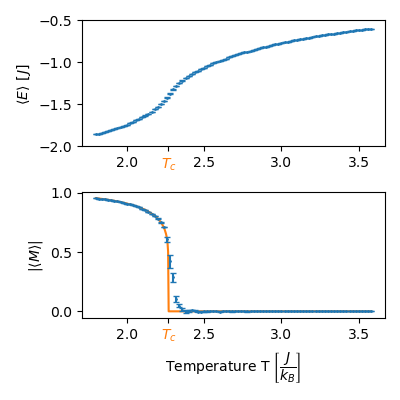
\includegraphics[width=.5\textwidth]{figs/fig2_EMplots.png}
		\caption{Mean energy (top) and absolute magnetization (bottom) per lattice site as computed by MCMC simulation at a range of temperatures. Data is drawn from 20 independent simulations: each data point is the magnitude of the average value of $M$ over all simulation steps; each standard error is the standard error of the mean of $M$ over all simulations, treating each $|M|$ as an independent measurement. Analytic $T_c$ (red) and analytic curves for $E$ and $M$ (green) as $N\rightarrow\infty$ are plotted for comparison.}
		\label{fig:fig2}
	\end{center}
\end{figure}

From $\Var{E}$ and $\Var{|M|}$ we calculate specific heat $c_V$ and magnetic susceptibility $\chi$ per lattice site:
\begin{align}
	c_V \equiv \frac{\partial \submin{E}}{\partial T} = & \frac{1}{k_BT^2}\frac{\Var{N^2 E}}{N^2} \label{eq:cv} \\
	\chi \equiv \frac{\partial \submin{M}}{\partial T} = & \frac{1}{k_BT}\frac{\Var{N^2 |M|}}{N^2}	\label{eq:chi}
\end{align}


By plotting $c_V$ and $\chi$ against temperature, we can observe the expected divergence of these quantities near $T_c$ (\autoref{fig:fig3}).

The analytical solution gives that $\chi$ and $c_V$ vary according to power laws near $T_c$. We use these relations to find $T_c$ and the critical exponents simultaneously, as multiple parameters in a single power law regression. We depict the resulting power law functions in \autoref{fig:fig3}.
We use only data from the shaded regions for the fits, where the inner radius is chosen based on convergence concerns near critical temperature\footnote{See Appendix A.} as well as finite size effects close to critical temperature, and the outer radius is chosen to include only data near $T_c$, where the power laws apply (i.e. the linear regime in \autoref{fig:fig5})[[fix me!]]. For the critical exponents defined both above and below $T_c$, we generate separate fits on each side [[fix me!]].

\begin{figure}[h]
	\begin{center}
		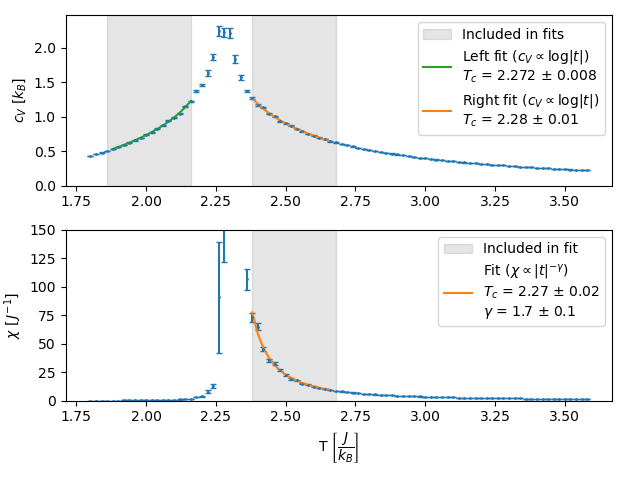
\includegraphics[width=.5\textwidth]{figs/fig3.png}
		\caption{Specific heat $c_V$ (top) and magnetic susceptibility $\chi$ (bottom) at a range of temperatures. $c_V$ and $\chi$ are calculated from variance in $E$ and $M$ respectively, as given in \autoref{eq:cv} and \autoref{eq:chi}. Each data point is the mean of $c_V$ or $\chi$ across 20 simulations at a given temperature, with error bars from the standard error of this mean. In the shaded regions, we use least-squares regression to fit expected functions (orange and green) near $T_c$ (logarithm for $c_V$, and a power law with critical exponent $\gamma$ for $\chi$), with $T_c$ as a free parameter. Although $\gamma$ is defined above and below $T_c$, finite size effects visible through high uncertainties in $\chi$ make it impractical to perform a second fit. Uncertainty in $T_c$ and $\gamma$ reflects uncertainty in the underlying data as well as the effect of small changes to each parameter on the $\chi^2$ value of the fit. [[fix me!]]}
		\label{fig:fig3}
	\end{center}
\end{figure}

We compute the spatial autocorrelation in spin states $\submin{\sigma_i\sigma_{i + x}}$ in the final lattice configuration of $20$ simulations for each temperature:
\begin{equation}
	\label{autocor}
	\submin{\sigma_i\sigma_{i + x}} = \frac{1}{N^2}\sum_{i, j} (\sigma_{(i, j)} - \bar{\sigma}_i)(\sigma_{(i, j + x)} - \bar{\sigma}_i)
\end{equation}
where the $i$ and $j$ vary over all rows and columns of the lattice. $\bar{\sigma}_i$ is the average spin in row/column $i$, and $j + x$ wraps around the lattice (i.e. is taken modulo $N$). For each temperature, we compute the mean autocorrelation across the $20$ trials and fit an exponential decay $\submin{\sigma_i\sigma_{i + x}} \propto e^{-x/\xi}$ (\autoref{fig:fig4a}), computing a value for the uncertainty in the length constant $\xi$ according to the variance in the autocorrelation across all trials. Here we take $\xi$ as the correlation length at that temperature. Correlation length clearly peaks near $T_c$ (\autoref{fig:fig4b}) as predicted analytically \cite{Onsager}. We fit a power law $\xi \propto |t|^{-\nu}$ to the data in the $t > 0$ portion of the annulus, with $T_c$ and $\nu$ as free parameters. We find $T_c = 2.32 \pm 0.03$ and $\nu = 0.6 \pm 0.1$, which deviate significantly from the analytical predictions $T_c \approx 2.269$, $\nu = 1$.

As an alternative method for determining the critical exponents $\alpha$, $\gamma$, $\beta$, and $\nu$, we plot $c_V$, $\log \chi$, and $\log |\submin{M}|$, and $\log \xi$ against $\log |t|$ (\autoref{fig:fig5}). In the case of $c_V$, the linearity with respect to $\log t$ supports the prediction $\alpha = 0$. For the latter three quantities, the transformed data yields a value for the corresponding critical exponent in the slope obtained by linear regression. We find $\gamma = 1.67 \pm .02$, $\beta = 0.097 \pm .001$, and $\nu = 0.76 \pm .04$. The reduced $\chi^2$ for the linear fit of $c_V$ is $1.553$.

\begin{figure}[h]
	\begin{center}
		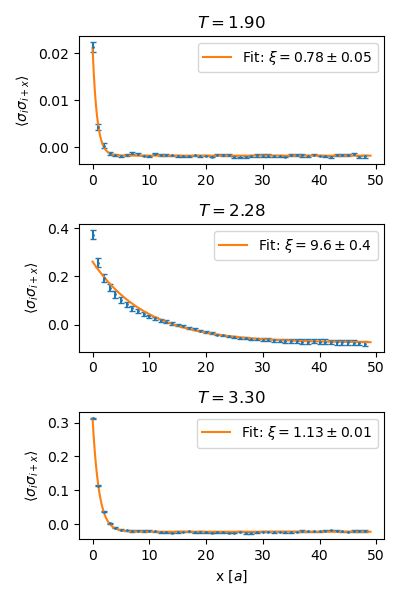
\includegraphics[width=.5\textwidth]{figs/fig4_autocors.png}
		\caption{Autocorrelation functions at representative temperatures: below, near, and above $T_c$. Shown in orange are exponential decay functions fit by least-squares regression to the positive portion of the autocorrelation data, with length scale parameter $\xi$. Autocorrelation frequently asymptotically approaches $\frac{-1}{N}$ (i.e. site become anticorrelated) after sufficient lattice distance, which likely plays a role in our calculation of $\nu$ far from the analytical value (see \textbf{discussion}). As with other fits, uncertainties in the fit value reflect both uncertainty in the underlying data, as well as the effect of changing fit parameters on the $\chi^2$ value of the fit. This can be seen above, where the uncertainty for $\xi$ in the middle graph is substantially greater than above and below, indicating data which does not conform to the expected exponential decay. Systematic error introduced by negative autocorrelations is not included in these error bars, and is discussed later.}
		\label{fig:fig4a}
	\end{center}
\end{figure}

\begin{figure}[h]
	\begin{center}
		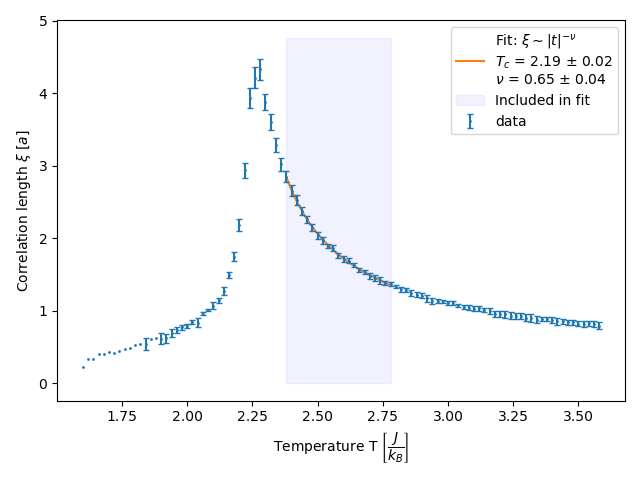
\includegraphics[width=.5\textwidth]{figs/fig4_xi.png}
		\caption{Correlation length $\xi$ at a range of temperatures. Data points are drawn from the fits depicted in \autoref{fig:fig4a}. As with $\chi$ and $c_v$, we fit a power law function (orange) to the data in the shaded region, with $T_c$ and $\nu$ as free parameters. Uncertainty in the fit parameters does not reflect systematic errors, leading to an inaccurate value for $T_c$, and a value for $\nu$ far from analytical predictions. [[Fix me!]]}
		\label{fig:fig4b}
	\end{center}
\end{figure}

\begin{figure*}[h]
	\begin{center}
		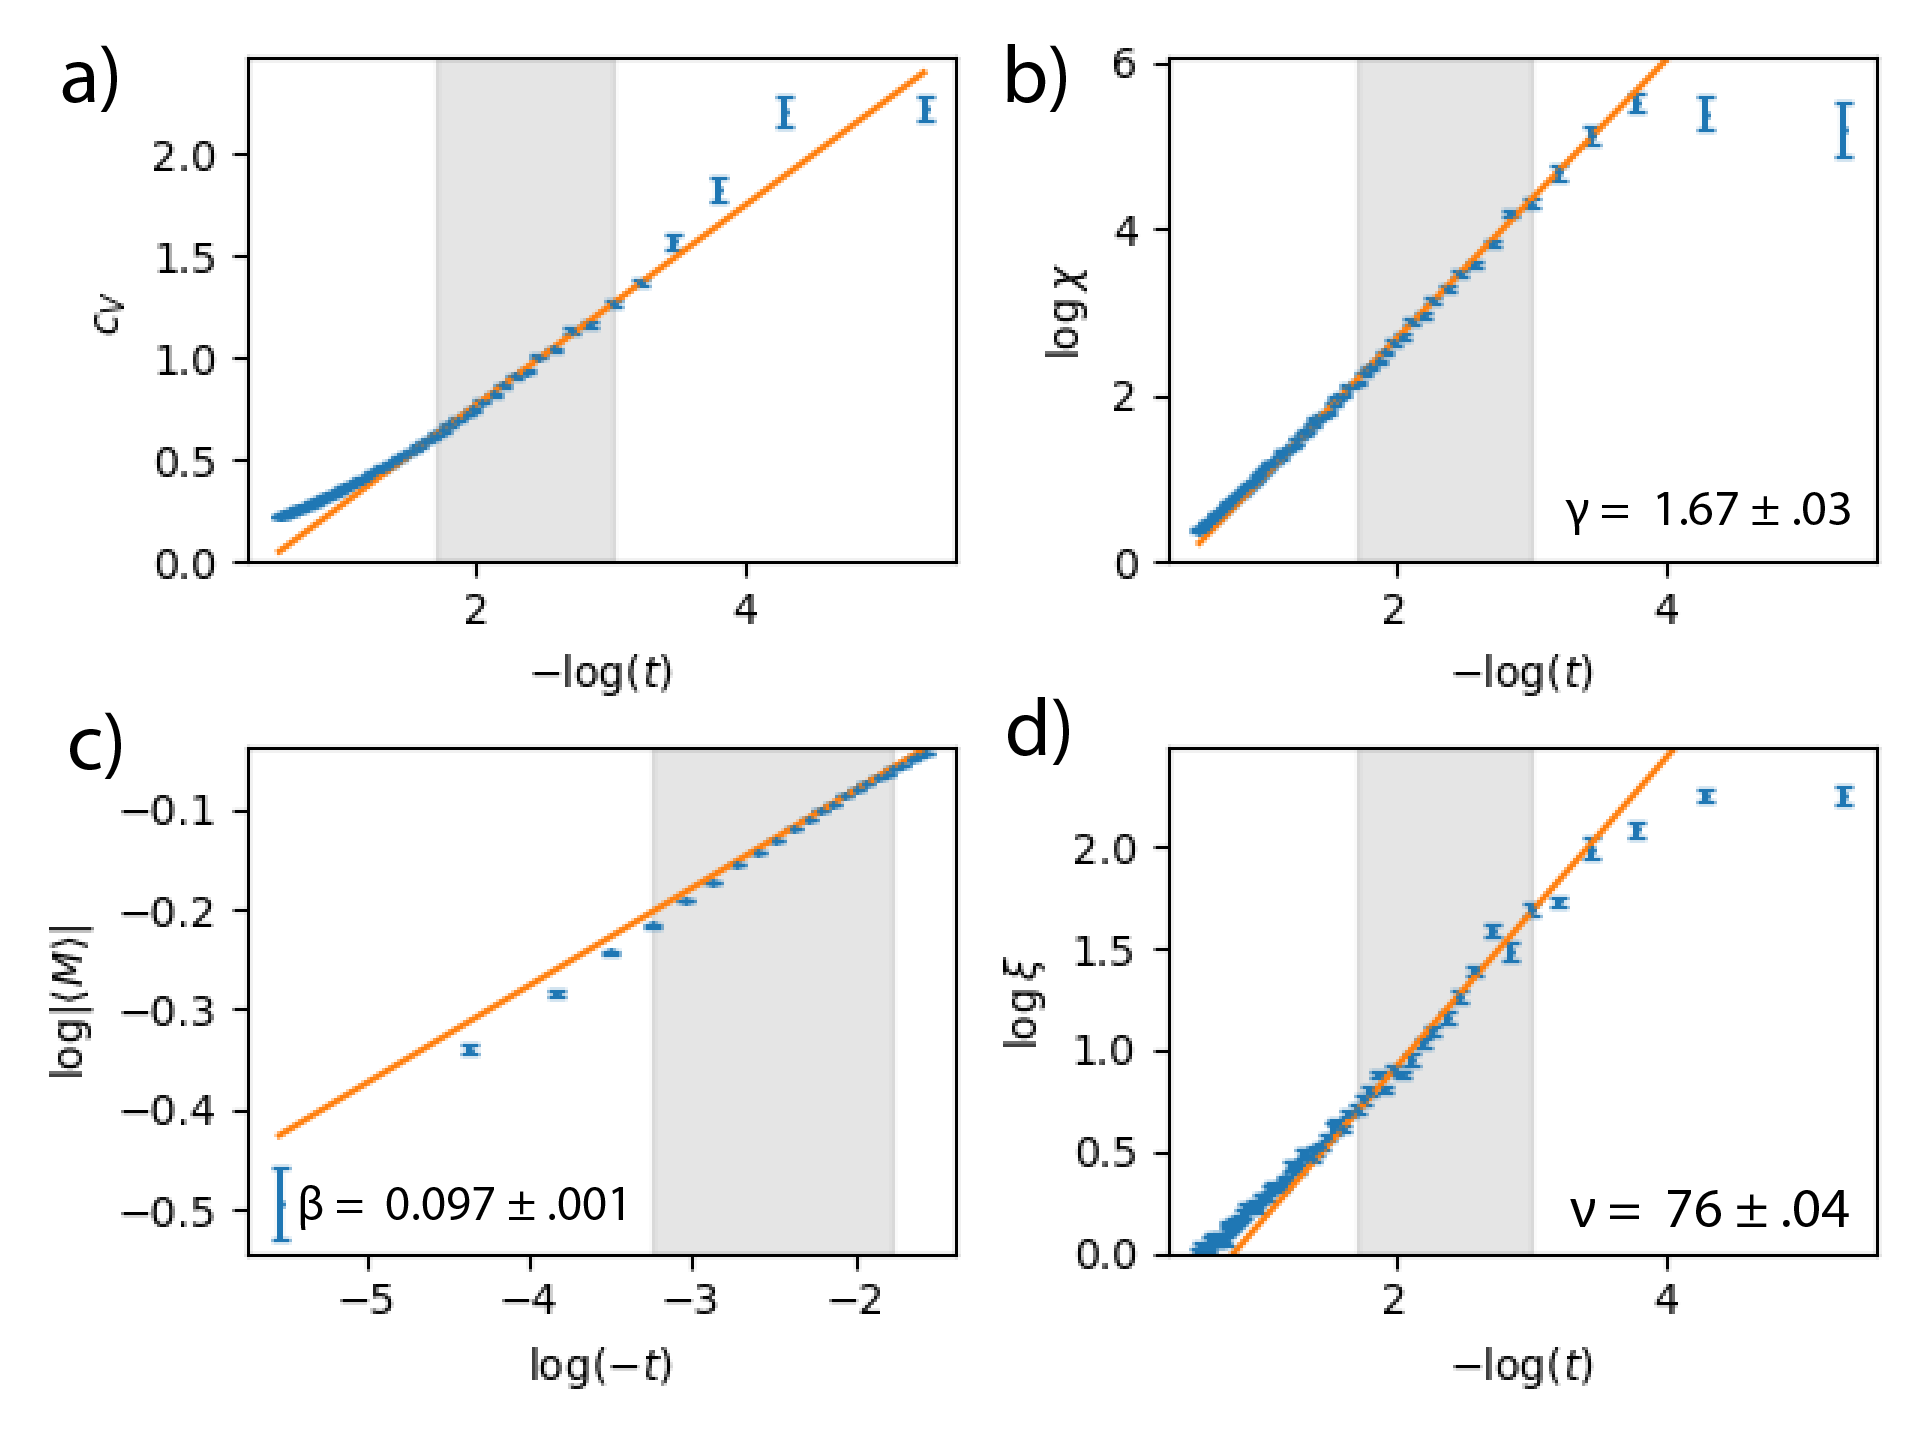
\includegraphics[width=1\textwidth]{figs/lastfig.png}
		\caption{Power law fits for the critical exponents for \textbf{a}. $c_V$ ($\alpha$), \textbf{b}. $\chi$ ($\gamma$), \textbf{c}. $|M|$ ($\beta$), and \textbf{d}. $\xi$ ($\nu$). We attempt to show $\alpha = 0$ by successfully fitting a logarithmic function to $c_V$. In each graph, the x-axis is $-\log{|t|}$, where normalized temperature $t = \frac{T - T_c}{T_c}$, and $T_c$ is the analytical value of $T_c$. We use data from temperatures above $T_c$ in all plots except \textbf{c}, as $\beta$ is not defined above $T_c$. As before, only data from the shaded regions was used for fits. We find the following values: $\gamma = 1.67 \pm .02$, $\beta = 0.097 \pm .001$, $\nu = 0.76 \pm .04$. For the fit in \textbf{a}, we calculated reduced $\chi^2 = 1.553$.}
		\label{fig:fig5}
	\end{center}
\end{figure*}

\textbf{Discussion:}

We see qualitative and quantitative evidence for a phase transition at the critical temperature. Values calculated for $T_c$ from $c_V$ and $\chi$ agree with one another and the analytical prediction, while the value calculated from $\xi$ disagrees dramatically. Given that all quantities not dependent on autocorrelation appear to experience a phase transition near the analytic $T_c$, this is almost certainly an issue with variables that go into $\xi$ specifically. Qualitative agreement of $\submin{E}$ and $|\submin{M}|$ with analytical predictions also lends strength to this claim.

What could be causing the discrepancy around $\xi$? One possibility is that the practice of using only the final lattice state in each simulation to calculate autocorrelation leads to a flawed measurement. However, this seems unlikely: if the flaw was simply too small a sample-size, we would expect to see high variance in autocorrelation over simulations, rather than the fairly tight uncertainties visible in \autoref{fig:fig4a}.

We also explored the possibility of some flaw in our autocorrelation algorithm, but in the end were unable to find such an issue, reaching the same results with multiple different implementations of the algorithm. The convergence to $\frac{-1}{N}$ rather than $0$ makes sense as a finite-size effect: it clearly approaches zero as $N \rightarrow \infty$. $\frac{-1}{N}$. One possible origin for such a term is the factor of $-\sigma_{(i, j)}/N$ in $\bar{\sigma}_i$. The negative autocorrelations near $T_c$, on the other hand, reflect the formations of islands with matching spins. With a lattice composed of several such islands, each lattice site is likely to share a spin with those around it, and have spin opposite to those farther away (rather than being merely uncorrelated). This anti-correlation does, however, call into question the validity of $\xi$ values calculated near $T_c$, since strong negative correlations do not resemble the exponential decay function used to fit for $\xi$. This is the most likely explanation for why our power law fit for $\xi$ produced unreliable values for $T_c$ and $\nu$.

We found the following critical exponents: $\gamma = 1.7 \pm .1$ ($T_c$ as free parameter) or $\gamma = 1.67 \pm .03$ ($T_c$ fixed to analytic value), $\beta = 0.097 \pm .001$, $\nu = 0.76 \pm .04$. We also find $\alpha = 0$ by cleanly fitting a logarithmic function to $c_V$. The critical exponents calculated with fixed $T_c$ (\autoref{fig:fig5}) do not fall within uncertainty of the expected analytic values, indicating either some systematic error or underestimates in uncertainty. Similarly, they do not quite satisfy Rushbrooke's or Josephson's identities from \autoref{eq:rushbrooke} and \autoref{eq:josephson}. One source of underestimated uncertainty is likely the fixed $T_c$: our calculated $T_c$ should be uncertain, and assuming a fixed $T_c$ eliminates this information.

\textbf{Acknowledgements:}
	We would like to thank Professor Nir Navon, Professor Laura Newburgh, and HongJoon Kim from the Yale Department of Physics for help running simulations and interpreting results. We would also like to thank the Phys 382L course staff for developing the Ising Model simulation code used throughout this paper.
	
\bibliographystyle{unsrt} 
\bibliography{refs}

\appendix
\section{Appendix A: Convergence}

\begin{figure}[h]
	\begin{center}
		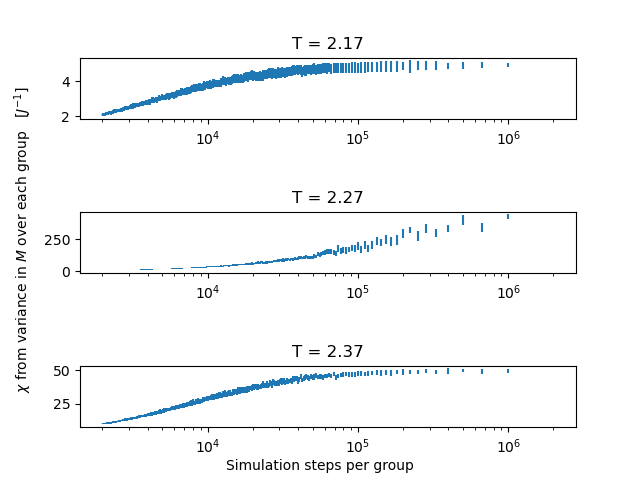
\includegraphics[width=.4\textwidth]{figs/figA1.png}
		\caption{$\chi$ values calculated with data from a simulation of 2,000,000 analyze steps. The total 2,000,000 steps were split as evenly as possible into groups of $n_{steps}$ (x axis), and variance in M was calculated across each group. Each data point is the average variance over all such groups.}
		\label{fig:figA1}
	\end{center}
\end{figure}

As stated under Methods, in order to faithfully represent the underlying distribution, the Metropolis-Hastings algorithm must arrive at the typical set, and then spend enough time in the typical set to reach a representative sample. We encountered issues with both aspects of convergence while collecting data.

The first issue was that at low temperatures, the simulation appeared to converge to states with large competing magnetic domains, rather than overall more aligned and thus lower-energy states. To clarify, this is not the experiment disagreeing with the theory, but rather a case of the MCMC algorithm not faithfully representing the desired distribution over a finite number of simulation steps. We solved this issue by annealing with an external magnetic field.

Annealing here refers to starting at a high temperature and magnetic field, and then slowly lowering them to the experimental values. The high temperature adds energy to the lattice, lowering the pull of local minima to allow the lattice to find overall lower-energy states. The initial magnetic field breaks the symmetry between positive and negative spin, pulling the lattice away from configurations with large magnetic domains and towards ultimately lower-energy states. 

As an example, consider a lattice initialized to be split in half down the middle, with the left half spin up, and the right half spin down. This state is significantly higher-energy than a lattice of all spin up, but reaching the uniform lattice requires passing through less-probable states. At low temperatures, this may not be possible, or might take an arbitrarily large number of steps. Similarly, with no external field, the two large domains might each grow in some places while ceding ground in others, preventing the overall lattice from reaching a more typical state.

In our simulations, we anneal from $T = 4 J/k_B$ and $B = .5 J$, linearly decreasing $T$ and $B$ to the experimental temperature and zero, respectively, over 3,000 steps. We then wait another 5,000 steps of "burn-in time," to allow transients from the extra temperature and field to dissipate.

The second issue we encountered was that we found $\chi$, and to a lesser extent $c_V$, to scale with simulation length, especially near $T_c$. This relationship is depicted in \autoref{fig:figA1}. At distance $.1 J/k_B$ from $T_c$ (top and bottom plots), we observe a region in which $\chi$ scales logarithmically with number of steps, followed by a plateau. On these plots, the plateau appears to begin near 100,000 steps. Very close to $T_c$, we do not find a plateau even within 2,000,000 steps.

We believe this effect is a function of local correlations over simulation steps. This is a normal feature of Metropolis sampling: the simulation traverses state space at a finite speed, and so lattice states at nearby steps are similar to one another. Near $T_c$, the set of typical states is larger, and so the simulation requires more steps to generate a representative sampling. $E$ and $M$ converge fairly quickly, but very close to $T_c$, $\chi$ and $c_V$ continue to correlate with number of steps well past even one million steps (see \autoref{fig:figA1}, middle plot).

One further piece of evidence for local correlations being at fault here is that if the simulation steps are \textit{shuffled} randomly (such that step 1 is no longer necessarily next to step 2, etc.), the relationship between number of steps and $\chi$ disappears. If we recreated \autoref{fig:figA1} with shuffled data, each graph would look like a horizontal line, with the y position of the $\chi$ value calculated using all 2,000,000 steps.

\end{document}
